\documentclass[a4paper]{article}
\usepackage{graphicx}
\usepackage{float}
\usepackage{pgfplots}
\pgfplotsset{compat=1.18}
\usepackage{listings}
\usepackage{enumitem}
\usepackage{cancel}
\usepackage{amsmath}
\usepackage{amssymb}
\usepackage{pgfplots}

\usepackage{tikz-cd}

\usetikzlibrary{decorations.pathreplacing} % for angle arc
\usetikzlibrary{angles, quotes, calc} % for drawing angles

\usepackage{color}   %May be necessary if you want to color links
\usepackage{hyperref}
\hypersetup{
    colorlinks=true, %set true if you want colored links
    linktoc=all,     %set to all if you want both sections and subsections linked
    linkcolor=black,  %choose some color if you want links to stand out
}

\usepackage{xcolor}
\usepackage[most]{tcolorbox}
% Define a custom tcolorbox environment for examples
\newtcolorbox{examplebox}[2][]{
  colback=blue!5!white,
  colframe=blue!30!black,
  title=#2,
  boxrule=0mm,
  fonttitle=\bfseries,
  width=\textwidth,
  breakable,
  #1
}
\newtcolorbox{definition} {
  colback=green!5!white,   % Background color
  colframe=green!75!black, % Border color
  title=Definizione,          % Title of the box
  boxrule=0.5mm,          % Thickness of the border                % Rounded corners
  fonttitle=\bfseries,    % Title font style
  width=\textwidth,       % Width of the box (adjustable)
}

\definecolor{codegreen}{rgb}{0,0.6,0}
\definecolor{codegray}{rgb}{0.5,0.5,0.5}
\definecolor{codepurple}{rgb}{0.58,0,0.82}
\definecolor{backcolour}{rgb}{0.95,0.95,0.92}

\lstdefinestyle{mystyle}{
    backgroundcolor=\color{backcolour},   
    commentstyle=\color{codegreen},
    keywordstyle=\color{magenta},
    numberstyle=\tiny\color{codegray},
    stringstyle=\color{codepurple},
    basicstyle=\ttfamily\footnotesize,
    breakatwhitespace=false,         
    breaklines=true,                 
    captionpos=b,                    
    keepspaces=true,                 
    numbers=left,                    
    numbersep=5pt,                  
    showspaces=false,                
    showstringspaces=false,
    showtabs=false,                  
    tabsize=2
}

\lstset{style=mystyle}

\makeatletter
\renewcommand*\env@matrix[1][*\c@MaxMatrixCols c]{%
  \hskip -\arraycolsep
  \let\@ifnextchar\new@ifnextchar
  \array{#1}}
\makeatother
\usepackage{tikz}
\usepackage{booktabs}
\title{Reti di calcolatori}
\author{Università di Verona\\Imbriani Paolo -VR500437\\Professor Damiano Carra}

\begin{document}

\begin{figure}
    \centering
    
\includegraphics[width=0.3\textwidth]{UniversityofVerona.png}
    \label{fig:centered-image}
\end{figure}

\maketitle 

\pagebreak

\tableofcontents

\pagebreak

\section{Introduzione}


Il problema principale che andremo ad affrontare nel corso è quello di permettere la comunicazione tra 2 calcolatori. Questo è possibile solo se le due macchine parlano la stessa "lingua". Gli strumenti e requisiti necessari sono i seguenti: 

\begin{enumerate}
    \item Un \textbf{protocollo} è un insieme di regole che sovraintende alla comunicazione, in cui si definiscono il formato dei messaggi e le azioni da intraprendere nel gestire i messaggi stessi
    \item \textbf{L'architettura di rete}, ovvero, come fisicamente questi messaggi verranno trasportati. 
\end{enumerate}
\begin{examplebox}{Esempio}
\textit{Immaginiamo che ci siano due utenti, A e B, che si vogliono mandare una lettera. Come si farebbe normalmente, una volta aver scritto la lettera, la si inserisce allì'interno di una busta che contiene informazioni importanti per la giusta riuscita della spedizione, ovverro l'indirizzo della consegna del messaggiio. Una volta fatto ciò, la si inserisce all'interno di una cassetta della posta affidandoci ai servizi di posta che porterà la lettera al destinatario e l'utente B finalmente recupera il messaggio.}
\end{examplebox}
La comunicazione tra due utenti è una catena di montaggio che costruisce e decostruisce l'informazione per permettere ai dati di viaggiare da un utente all'altro. Quali sono le tecniche di instradamento necessario per far viaggare il messaggio in rete? 
Affronteremo questo tipo di comunicazione attraverso l'approccio topdown ovvero partendo dal livello più alto (quello riferito al layer dell'applicazione) fino ad arrivare a quello fisico e più basso.

\section{Architetture di Rete}

Distinguiamo diversi elementi di base che fanno parte di un architettura di rete:

\begin{itemize}
    \item Calcolatori (End-host)
    \item Router (Intermediate host) 
    \item Collegamenti
\end{itemize}
Il router è quell'apparrato che decide quale strada il pacchetto deve fare per raggiungere il destinatario. La LAN (Local Area Network, Rete locale) è caratterizzata dal fatto che al suo interno contiene gli end-host. La backbone tipicamente contiene specificatemente gli apparati in una topologia che decide il gestore della rete stessa. La differenza tra le due è che nella LAN ci sono gli end-host mentre nel backbone si trovano solo collegamenti tra gli apparati che permettono il viaggio dei messaggi sul territorio.
\\\\
Quindi, una prima definizione di Internet è possibile farla grazie a questi elementi: infatti se dovessimo astrarla ad alto livello, ci sono varie LAN collegate tramite il backbone (dove tipicamente la tecnologia utilizzata è quella cablata, al contrario delle LAN dove è un mix tra cablata e wireless).

\subsection{Com'è organizzato il backbone?}

Tramite l'ISP (Internet Service Provider) che appunto posseggono una parte di rete e che permettono di farla usufruire agli utenti.

\begin{itemize}
    \item Livello 1: Estensione Internazionale (Copre diverse nazioni) 
    \item Livello 2: Lavorano a livello nazionale
    \item Livello 3: Locale
\end{itemize}

Tipicamente proprio come dei router di bordo, gli ISP di livello 1 sono collegati a loro volta altri ISP di livello 1. Questo permette agli utenti di collegarsi a diversi ISP di livello 1 anche se molto lontani tra loro. Globalmente quindi: 
\begin{definition}
  \textit{Internet è un insieme di reti organizzato gerarchicamente.}  
\end{definition}
Per raggiungere un utete, in genere si segue un percorso gerarchico. Ma ovviamente la scelta del percorso segue criteri basati su:

\begin{enumerate}
    \item distanza
    \item tempo
\end{enumerate}
Non necessariamente il percorso più breve è quello più veloce o viceversa. Il discorso delle migliore tecniche di instradamento verranno spiegeate più avanti nel corso.

\subsection{Modalità di trasferimento dell'informazione tra due utenti}

Ci sono due opzioni: 
\begin{itemize}
    \item Reti a commutazione di circuito
    \item Reti a commutazione di pacchetto
\end{itemize}

\subsubsection{Commutazione di circuito}

Le risorse (capacità del canale di trasmissione) vengono riservate end-to-end per la communicazione. \textbf{Viene riservato un circuito }che viene utilizzato dai due utenti. Quindi per esempio, nel momento che viene effettuata una chiamata, viene riservato un canale dove fino alla fine della chiamata rimarrà occupato. Quindi ci sarà una porzione di tempo dove il circuito verrà instarauto (ritardo) e poi il messaggio è pronto per essere trasmesso.
\\\\Pro: 
\begin{itemize}
    \item Risorse dedicate
    \item Ritardo deterministico
\end{itemize}
Contro:
\begin{itemize}
    \item nel caso di utilizzo sporadico, ho uno spreco di risorse
\end{itemize}
\subsubsection{Commutazione di pacchetto}

L'informazione (o messaggio) viene suddiviso in \textbf{pacchetti}. Ad ogni pacchetto viene aggiunta un'intestazione per permettere la consegna del pacchetto stesso e la ricostruzione del messaggio. Il messaggio viene spezzato in unità più piccole e a ciascuna di queste unità viene aggiunta un intestazione che ha almeno due scopi:
\begin{enumerate}
    \item Rendere indipendenti questi singoli pacchetti in maniera che possano essere spediti separatamente. 
    \item Specificare l'ordine delle unità per andare a ricostruire il messaggio.
\end{enumerate}
Il router in base all'intestazione che possiede il pacchetto sa in che direzione spedirli ed ecco perché sono liberi di essere trasmessi in maniera indipendente. Il messaggio può anche arrivare fuori sequenza che tanto verrebbe ricostruito nel giusto ordine.
\\\\
Pro:
\begin{itemize}
    \item Uitlizza le risorse solo quando ha pacchetti da trasmettere. 
    \item Multiplazione statistica, ovvero vado a mettere insieme pacchetti che vengono da fonti diverse
\end{itemize}
Contro:
\begin{itemize}
    \item Potenziale perdita dei pacchetti 
    \item Ritardi aumentati che dipende dal numero di Router attraversati lungo il viaggio del pacchetto
\end{itemize}
Il router adotta la tecnica del \textit{Store $\&$ Forward} ovvero prima memorizza l'intero pacchetto, leggere l'intestazione e in base alla destinazione decidi quale è il successivo router a cui mandare il pacchetto. 

\subsection{Ritardi di trasmissione}

Come abbiamo già visto, tramite lo Store $\&$ Forward la commutazione a pacchetto introduce la possibilità che i messaggi arrivino in ritardo. Si può dividere in diverse componenti: 
\begin{enumerate}
    \item Ritardo di elaborazione al nodo. Il router deve semplicemente decidere quale uscita instradare per il messaggio.
    \item Ritardo di accodamento (tempo speso nel buffer prima che il pacchetto venga trasmesso) ed è la componente principale (ordine di grandezza decisamente più grande rispetto a quello dell'elaborazione del nodo)
    \item Ritardo di trasmissione $\rightarrow \frac{\text{Grandezza messaggio}}{\text{ Grandezza del canale}}$
    \item Ritardo di propagazione
\end{enumerate}
Tuttavia vogliamo chiederci quale sia effettivamente l'ordine di grandezza del ritardo? 
Possiamo distinguere tra i tipi di destinazione:
\begin{itemize}
    \item locale (fondamentalmente nella stessa nazione, dove è $< 10 ms$) 
    \item internazionale ($20-40 ms$)
    \item intercontinentale ($> 100 ms$)
\end{itemize}
Quali sono gli strumenti che misurando il ritardo end-to-end tra una sorgente e una destinazione? 
\begin{itemize}
    \item Il primo strumento è il ping. Dati 2 utenti e 2 diverse, viene inviato un messaggiod di ping e capire il tempo che intercorre tra l'invio del messaggio di ping e la ricezione della risposta (\textit{echo reply}). Questo tempo viene chiamato \textit{Round-trip-time}. Questo tempo stima il ritardo complessivo per raggiungere l'utente e ricevere la risposta. Non è detto che il tempo sia simmetrico o asimmetrico. 
    \item Traceroute, dati 2 utenti manda dei messaggi anche ai router intermedi. È un ping potenziato dove controlla il ritardo anche tra i router intermedi. 
\end{itemize}
Quante informazioni riesco a trasmettere? $\frac{bit}{s}$
\\\\Questa informazione dipende dalle capacità di tutti i canali di trasmissione attraversati
La banda end-to-end a disposizione viene definito "\textit{troughput}" ed è determinato dal collo di bottiglia. 


\section{Modello a strati}
Il modello a strati affronta la \textbf{comunicazione tra due entità} secondo la modalità
\textbf{divide et impera}.
\begin{figure}[H]
  \centering
  % \includegraphics[width=0.70\textwidth]{comunicazione}
\end{figure}
Per scambiare informazioni le due entità devono comunicare. La comunicazione si divide in:
\begin{itemize}
  \item \textbf{Comunicazione logica}: Gestisce le problematiche relative all'informazione

    \noindent Ad esempio:
    \begin{itemize}
      \item Linguaggio utilizzato
      \item Come comportarsi nello scambio
    \end{itemize}

  \item \textbf{Comunicazione Fisica}: Come trasferire i diversi bit. Il contenuto
    dell'informazione non è importante.
\end{itemize}

\begin{figure}[H]
  \centering
  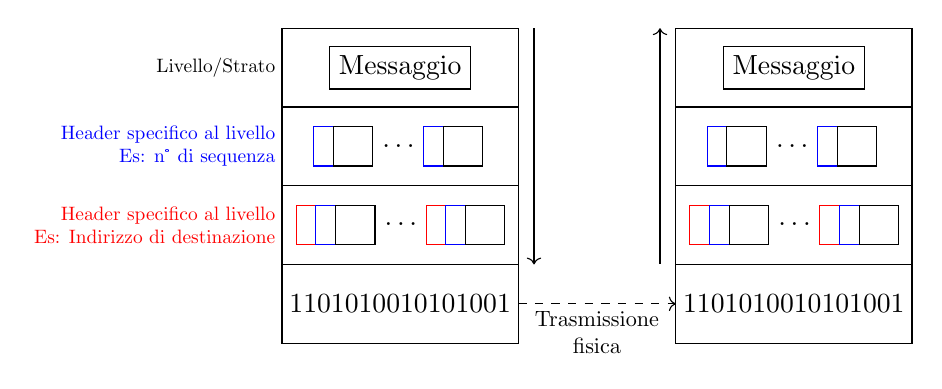
\begin{tikzpicture}
    \draw (0,0) rectangle ++(3,-1) node[midway,draw] {Messaggio};
    \node[left,align=right,scale=0.7] at (0,-0.5)
      {Livello/Strato};

    \draw (0,-1) rectangle ++(3,-1);
    \node[blue,left,align=right,scale=0.7] at (0,-1.5)
      {Header specifico al livello\\Es: n° di sequenza};

    \draw (0,-2) rectangle ++(3,-1);
    \node[red,left,align=right,scale=0.7] at (0,-2.5)
      {Header specifico al livello\\Es: Indirizzo di destinazione};

    \draw (0,-3) rectangle ++(3,-1) node[midway] {$1101010010101001$};

    \coordinate (r1) at (0.4,-1.75);
    \draw[red] (r1) rectangle ++(0,0.5);
    \draw[blue] (r1) ++(0,0.5) rectangle ++(0.25,-0.5);
    \draw (r1) ++(0,0.5) ++(0.25,-0.5) rectangle ++(0.5,0.5) node[below right,yshift=-0.1cm] {$\ldots$};

    \coordinate[right of=r1, xshift=0.4cm] (r2);
    \draw[red] (r2) rectangle ++(0,0.5);
    \draw[blue] (r2) ++(0,0.5) rectangle ++(0.25,-0.5);
    \draw (r2) ++(0,0.5) ++(0.25,-0.5) rectangle ++(0.5,0.5);


    \coordinate (r3) at (0.18,-2.75);
    \draw[red] (r3) rectangle ++(0.25,0.5);
    \draw[blue] (r3) ++(0.25,0.5) rectangle ++(0.25,-0.5);
    \draw (r3) ++(0.25,0.5) ++(0.25,-0.5) rectangle ++(0.5,0.5) node[below right,yshift=-0.1cm] {$\ldots$};

    \coordinate[right of=r3, xshift=0.65cm] (r4);
    \draw[red] (r4) rectangle ++(0.25,0.5);
    \draw[blue] (r4) ++(0.25,0.5) rectangle ++(0.25,-0.5);
    \draw (r4) ++(0.25,0.5) ++(0.25,-0.5) rectangle ++(0.5,0.5);

    \draw[->] (3.2,0) -- ++(0,-3);



    \draw (5,0) rectangle ++(3,-1) node[midway,draw] {Messaggio};
    \draw (5,-1) rectangle ++(3,-1);
    \draw (5,-2) rectangle ++(3,-1);

    \draw (5,-3) rectangle ++(3,-1) node[midway] {$1101010010101001$};

    \coordinate (r1) at (5.4,-1.75);
    \draw[red] (r1) rectangle ++(0,0.5);
    \draw[blue] (r1) ++(0,0.5) rectangle ++(0.25,-0.5);
    \draw (r1) ++(0,0.5) ++(0.25,-0.5) rectangle ++(0.5,0.5) 
      node[below right,yshift=-0.1cm] {$\ldots$};

    \coordinate[right of=r1, xshift=0.4cm] (r2);
    \draw[red] (r2) rectangle ++(0,0.5);
    \draw[blue] (r2) ++(0,0.5) rectangle ++(0.25,-0.5);
    \draw (r2) ++(0,0.5) ++(0.25,-0.5) rectangle ++(0.5,0.5);


    \coordinate (r3) at (5.18,-2.75);
    \draw[red] (r3) rectangle ++(0.25,0.5);
    \draw[blue] (r3) ++(0.25,0.5) rectangle ++(0.25,-0.5);
    \draw (r3) ++(0.25,0.5) ++(0.25,-0.5) rectangle ++(0.5,0.5) 
      node[below right,yshift=-0.1cm] {$\ldots$};

    \coordinate[right of=r3, xshift=0.65cm] (r4);
    \draw[red] (r4) rectangle ++(0.25,0.5);
    \draw[blue] (r4) ++(0.25,0.5) rectangle ++(0.25,-0.5);
    \draw (r4) ++(0.25,0.5) ++(0.25,-0.5) rectangle ++(0.5,0.5);

    \draw[<-] (4.8,0) -- ++(0,-3);

    \draw[->,dashed] (3,-3.5) -- ++(2,0) node[midway,below,align=center,scale=0.8] {Trasmissione\\fisica};
  \end{tikzpicture}
  \caption{Comunicazione tra due entità}
\end{figure}
\noindent
Ad ogni \textbf{livello} (o strato) viene elaborata parzialmente l'informazione e
trasformata. Ogni livello aggiunge un \textbf{header} che contiene un'informazione
specifica a quel livello, seguendo un \textbf{protocollo} (specifico per quel livello).

\vspace{1em}
\noindent
Ogni livello ha uno o più protocolli associati, e l'insieme dei protocolli di tutti i
livelli è chiamato \textbf{stack protocollare}.

\subsection{Stack ISO/OSI}
Il modello \textbf{ISO/OSI} (International Standard Organization / Open System Interconnection)
definisce dei livelli a seconda del sistema:
\begin{itemize}
  \item \textbf{End system}:
    \begin{figure}[H]
      \centering
      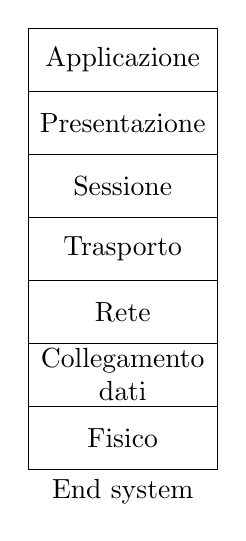
\begin{tikzpicture}[scale=0.8]
        \draw (0,6) rectangle ++(3,1) node[midway] {Applicazione};
        \draw (0,5) rectangle ++(3,1) node[midway] {Presentazione};
        \draw (0,4) rectangle ++(3,1) node[midway] {Sessione};
        \draw (0,3) rectangle ++(3,1) node[midway] {Trasporto};
        \draw (0,2) rectangle ++(3,1) node[midway] {Rete};
        \draw (0,1) rectangle ++(3,1) node[midway,align=center] {Collegamento\\dati};
        \draw (0,0) rectangle ++(3,1) node[midway] {Fisico};
        \node[below] at (1.5,0) {End system};
      \end{tikzpicture}
      \caption{Stack ISO/OSI per l'end system}
    \end{figure}
  \item \textbf{Intermediate system}:
    \begin{figure}[H]
      \centering
      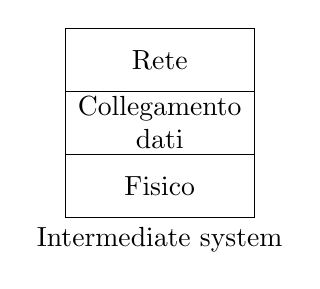
\begin{tikzpicture}[scale=0.8]
        \draw (0,2) rectangle ++(3,1) node[midway] {Rete};
        \draw (0,1) rectangle ++(3,1) node[midway,align=center] {Collegamento\\dati};
        \draw (0,0) rectangle ++(3,1) node[midway] {Fisico};
        \node[below] at (1.5,0) {Intermediate system};
      \end{tikzpicture}
      \caption{Stack ISO/OSI per l'intermediate system}
    \end{figure}
\end{itemize}

\subsection{Stack TCP/IP}
Nella pratica (rete Internet) si utilizza lo stack protocollare \textbf{TCP/IP}:
\begin{itemize}
  \item \textbf{End system}:
    \begin{figure}[H]
      \centering
      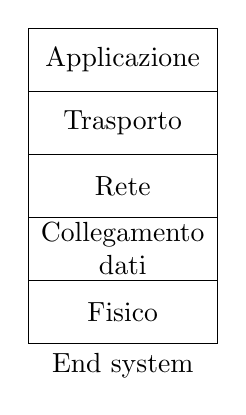
\begin{tikzpicture}[scale=0.8]
        \draw (0,4) rectangle ++(3,1) node[midway] {Applicazione};
        \draw (0,3) rectangle ++(3,1) node[midway] {Trasporto};
        \draw (0,2) rectangle ++(3,1) node[midway] {Rete};
        \draw (0,1) rectangle ++(3,1) node[midway,align=center] {Collegamento\\dati};
        \draw (0,0) rectangle ++(3,1) node[midway] {Fisico};
        \node[below] at (1.5,0) {End system};
      \end{tikzpicture}
      \caption{Stack TCP/IP per l'end system}
    \end{figure}
  \item \textbf{Intermediate system}:
    \begin{enumerate}
      \item Rete
      \item Collegamento dati
      \item Fisico
    \end{enumerate}
    \begin{figure}[H]
      \centering
      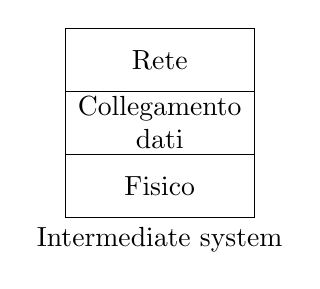
\begin{tikzpicture}[scale=0.8]
        \draw (0,2) rectangle ++(3,1) node[midway] {Rete};
        \draw (0,1) rectangle ++(3,1) node[midway,align=center] {Collegamento\\dati};
        \draw (0,0) rectangle ++(3,1) node[midway] {Fisico};
        \node[below] at (1.5,0) {Intermediate system};
      \end{tikzpicture}
      \caption{Stack TCP/IP per l'intermediate system}
    \end{figure}
\end{itemize}

\noindent
Il nome deriva dai due principali protocolli utilizzati:
\begin{itemize}
  \item Protocollo di trasporto: \textbf{TCP} (Transport Control Protocol)
  \item Protocollo di rete: \textbf{IP} (Internet Protocol)
\end{itemize}

\subsection{Entità coinvolte nella comunicazione}
Su un calcolatore possono girare più applicazioni. Ogni applicazione
può avere una connessione attiva, quindi ci possono essere più connessioni
attive contemporaneamente.

\vspace{1em}
\noindent
Un applicazione può avere più istanzee di comunicazione, cioè più connessioni
attive contemporaneamente.

\vspace{1em}
\noindent
Di conseguenza \textbf{l'istanza di un'applicazione} è la vera e propria entità
all'interno di una comunicazione. Quando si parla di entità si fa riferimento a uno
specifico processo che gira su un calcolatore

\subsubsection{Identificazione dei processi}
Per identificare un processo servono 2 informazioni:
\begin{enumerate}
  \item \textbf{Indirizzo IP}: Identifica il calcolatore
  \item \textbf{Porta}: Codice numerico che identifica il processo all'interno del 
    calcolatore
\end{enumerate}
\begin{figure}[H]
  \centering
  % \includegraphics[width=0.7\textwidth]{comunicazione-processi}
  \caption{Comunicazione tra processi}
\end{figure}
Un flusso di comunicazione è identificato univocamente dalla tupla:
\[
  (IP_A, IP_B, Porta_A, Porta_B)
\]
La porta viene assegnata ad un processo soltanto quando esso inizia a comunicare.

\subsubsection{Ottenimento dell'IP e della porta}
Queste informazioni sono contenute negli header aggiunti ad ogni livello.
\begin{figure}[H]
  \centering
  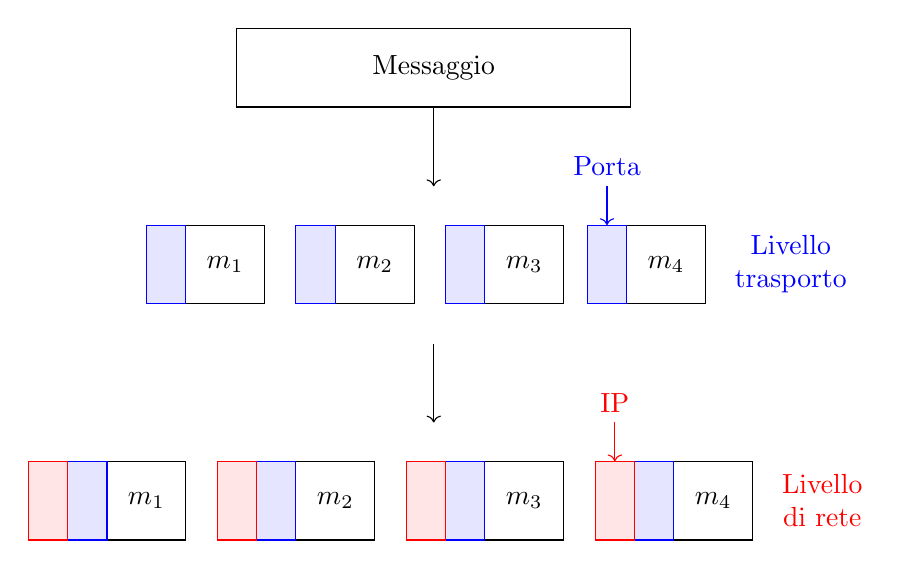
\begin{tikzpicture}
    \node[draw, minimum width=5cm, minimum height=1cm] at (0.45,0) (m) {Messaggio};
    \draw[->] (m.south) -- ++(0,-1);

    \coordinate (a) at (-2.7,-3);
    \draw (a) rectangle ++(1,1) node[midway] {$m_1$};
    \draw[blue,fill, fill opacity=0.1] (a) ++(0,1) rectangle ++(-0.5,-1);

    \coordinate (b) at (-0.8,-3);
    \draw (b) rectangle ++(1,1) node[midway] {$m_2$};
    \draw[blue,fill, fill opacity=0.1] (b) ++(0,1) rectangle ++(-0.5,-1);

    \coordinate (c) at (1.1,-3);
    \draw (c) rectangle ++(1,1) node[midway] {$m_3$};
    \draw[blue,fill, fill opacity=0.1] (c) ++(0,1) rectangle ++(-0.5,-1);

    \coordinate (d) at (2.9,-3);
    \draw (d) rectangle ++(1,1) node[midway] {$m_4$};
    \draw[blue,fill, fill opacity=0.1] (d) ++(0,1) rectangle ++(-0.5,-1);
    \draw[<-,blue] (d) ++(-0.25,1) -- ++(0,0.5) node[above,blue] {Porta};
    \draw[blue] (d) ++(1.25,0.5) node[right,align=center] {Livello\\trasporto};

    \draw[->] (m.south) ++(0,-3) -- ++(0,-1);

    \coordinate (e) at (-3.7,-6);
    \draw (e) rectangle ++(1,1) node[midway] {$m_1$};
    \draw[blue,fill, fill opacity=0.1] (e) ++(0,1) rectangle ++(-0.5,-1);
    \draw[red,fill, fill opacity=0.1] (e) ++(-0.5,1) rectangle ++(-0.5,-1);

    \coordinate (f) at (-1.3,-6);
    \draw (f) rectangle ++(1,1) node[midway] {$m_2$};
    \draw[blue,fill, fill opacity=0.1] (f) ++(0,1) rectangle ++(-0.5,-1);
    \draw[red,fill, fill opacity=0.1] (f) ++(-0.5,1) rectangle ++(-0.5,-1);

    \coordinate (g) at (1.1,-6);
    \draw (g) rectangle ++(1,1) node[midway] {$m_3$};
    \draw[blue,fill, fill opacity=0.1] (g) ++(0,1) rectangle ++(-0.5,-1);
    \draw[red,fill, fill opacity=0.1] (g) ++(-0.5,1) rectangle ++(-0.5,-1);

    \coordinate (h) at (3.5,-6);
    \draw (h) rectangle ++(1,1) node[midway] {$m_4$};
    \draw[blue,fill, fill opacity=0.1] (h) ++(0,1) rectangle ++(-0.5,-1);
    \draw[red,fill, fill opacity=0.1] (h) ++(-0.5,1) rectangle ++(-0.5,-1);
    \draw[<-,red] (h) ++(-0.75,1) -- ++(0,0.5) node[above,red] {IP};
    \draw[red] (h) ++(1.25,0.5) node[right,align=center] {Livello\\di rete};

  \end{tikzpicture}
  \caption{Porta e IP}
\end{figure}

\noindent
Un pacchetto si può rappresentare nel seguente modo:
\begin{figure}[H]
  \centering
  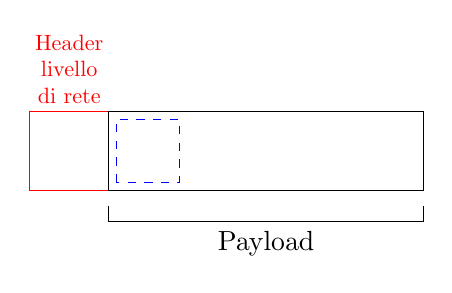
\begin{tikzpicture}
    \draw[red] (0,0) rectangle ++(1,1);
    \node[red,above,scale=0.8,align=center] at (0.5,1) {Header\\livello\\di rete};

    \draw[dashed,blue] (0,0) ++(1.1,0.1) rectangle ++(0.8,0.8);
    \draw (0,0) ++(1,0) rectangle ++(4,1);

    \draw (0,0) ++(1,-0.2) -- ++(0,-0.2) -- ++(4,0) node[midway,below] {Payload}
      -- ++(0,0.2);
  \end{tikzpicture}
  \caption{Rappresentazione di un pacchetto}
\end{figure}

\pagebreak

\section{Indirizzi IP}
Sono identificativi \textbf{univoci} di un'interfaccia di un host della rete Internet.
Un end system può avere soltanto un'interfaccia, ma un router deve avere minimo 2
interfacce per poter permettere la comunicazione tra più entità.


\begin{examplebox}{Esempio}
  Un esempio di indirizzo IP è:
  \[
    10011101 \;\; 00011011 \;\; 0001 \; 0011 \;\; 0111 \; 1011
  \] 
  Per facilitare la lettura e la gestione degli indirizzi IP si usa la notazione
  \textbf{decimale puntata}. In questa notazione si considerano blocchi di 8 bit, di
  conseguenza si avranno 4 blocchi. Ogni blocco viene tradotto in un numero intero decimale
  compreso tra 0 e 255 e separato da un punto:
  \[
    157.27.19.123
  \] 
\end{examplebox}

\subsection{Suddivisione dei bit}
I bit dell'indirizzo IP hanno tutti la stessa importanza?

\vspace{1em}
\noindent
Prendiamo ad esempio i numeri telefonici della rete fissa:
\[
  \underbrace{0039 \; 045 \; 802}_{\text{Prefisso}} \; \underbrace{7059}_{\text{Suffisso}}
\] 
\begin{itemize}
  \item Il prefisso è l'identificativo di una specifica organizzazione
  \item Il suffisso identifica un utente specifico all'interno dell'organizzazione
\end{itemize}

\vspace{1em}
\noindent
Allo stesso modo in un indirizzo IP si ha \textbf{prefisso} e \textbf{suffisso}
\begin{itemize}
  \item \textbf{Prefisso}: Identifica una rete specifica
  \item \textbf{Suffisso}: Identifica un'interfaccia di un host di una specifica rete 
\end{itemize}

\subsubsection{Identificazione del prefisso e del suffisso}
Nel caso dei numeri telefonici si inserisce una barra per separare il prefisso dal suffisso:
\[
  045/7021412
\]
Negli indirizzi IP il numero di bit dedicati al prefisso dipende dalla dimensione della
rete ed è indicato da una barra seguita da un numero.
\[
  157.27.19.123/16
\] 
Significa che i primi 16 bit dell'indirizzo IP sono dedicati al prefisso.


\subsection{Come suddividere gli indirizzi}


Quanti indirizzi per gli host contiene una rete e ha un prefisso/$n$?

\[
    \overbrace{10011101 \;\; 00011011 \;\; 0001 \; 0011 \;\; 0111 \; 1011}^{32 bit}
\] 

\[\# \text{ indirizzi} \rightarrow 2^{32-n}\]
\begin{examplebox}{Esempio}
\[n = 20 \rightarrow 2^{12} = 4096\]
\[n = 24 \rightarrow 2^8 = 256\]
\end{examplebox}
In base al numero di indirizzi che devo riservare devo capire quale tipo di suffisso mi riesca a sostenere il numero di host.

\subsubsection{Indrizzi IP riservati}
\begin{enumerate}
    \item \textbf{This host} \[0000 \;\; \dots \; \; 0000 \rightarrow 0.0.0.0\]
    \item \textbf{Local/Limited Broadcast } \[ \underbrace{1111 \;\; \dots \; \; 1111}_{\text{32 bit a 1}} \rightarrow 255.255.255.255\]
    \item \textbf{Indirizzo di rete} \[ \underbrace{1010100010}_{\text{n prefisso}} \underbrace{00000000}_{\text{32-n bit a 0}}\]
    indirizzo con il quale viene identificata la rete
    \item \textbf{Directed Broadcast} \[ \underbrace{1010100010}_{\text{n prefisso}} \underbrace{11111111}_{\text{32-n bit a 1}}\] 
    indirizzo con il quale viene identificato il broadcast alla rete
\end{enumerate}

\subsection{Subnet Mask}

\textit{Come faccio a conoscere il mio indirizzo IP e la dimensione del prefisso della rete a cui sono collegato? }
\\\\
L'indirizzo IP e la dimensione del prefisso dipendono dalla rete a cui sono collegato.
Per conoscere il proprio indirizzo IP si utilizza il comando "ifconfig".
\begin{center}
Sul mio Mac in questo momento ho l'indirizzo:\\
Indirizzo: $157.27.201.95/?$\\
Netmassk: 0xFFFFF000\\
Broadcast: $157.27.207.255$
\end{center}
Per identificare il $\#$ host del prefisso i calcolatori:
\begin{examplebox}{Esempio}
\[/16 \Longrightarrow 1111 1111 1111 1111 0000 0000 0000 \; \; ... \; \; 0000\]
Questa sequenza è chiamata \textbf{"maschera"} ed è una sequenza che viene abbinata all'indirizzo IP
\begin{center}
    IP: $101010010101001 \; \; ... \; \; 10100100$
    \\
    Mask: $\underbrace{111111 .... 11111}_{\text{prefisso}}\; \; \underbrace{0000 ... 0000}_{\text{suffisso}}$ \\
    IP $\&$ Mask si ottiene all'indirizzo di rete a cui quell'indirizzo IP appartiene
\end{center}
\end{examplebox}
La maschera può essere rappresentata:
\begin{itemize}
    \item Notazione decimale
    \item Notazione esadecimale
\end{itemize}

\subsubsection{Notazione Esadecimale}

Gruppi di 4 bit.

\[\begin{matrix}
    0000 \rightarrow 0\\
    0001 \rightarrow 1\\
    0010 \rightarrow 2\\
    \vdots\\
    1111 \rightarrow F
\end{matrix}\]
\[2^4 \text{ configurazioni} \rightarrow 16 \text{ simboli}\]
Il simbolo "$0x$" vuol dire che sta rappresentando con la notazione esadecimale:
\begin{examplebox}{Esempio}
    
\[0xFFFFF000 \rightarrow \underbrace{1111  \; \; 1111 \; \; 1111 \; \; 1111  \; \;1111}_{20} \; \; \underbrace{0000  \; \;0000 \; \; 0000}_{12}\]
Quindi la rete a cui sono connesso è $/20$.
\end{examplebox}
Altre inforamzioni sulla rete (dato un indirizzo IP si possono ottenere con il calcolo "\textit{whois}"
\\\\
\textit{Perché ifconfig dice che il mio indirizzo è associato ad una rete /20, mentre whois dice che è associata ad una rete /16?}
\\\\
Per "ifconfig" 
\[\underbrace{1010010101010100}_{20 \text{ prefisso}} \;\; ... \; \; 0100 \rightarrow 2^{32-20} \rightarrow 2^{12} = 4096 \text{ indirizzi}\]
Per "whois"
\[\underbrace{1000100001000100}_{16 \text{ prefisso}} \;\; ... \; \; 0100 \rightarrow 2^{32-16} \rightarrow 2^{16} = 65536 \text{ indirizzi}\]
Questo è dovuto al \textbf{SUBNETTING}. Dove la rete più grande (UNIVR) ha diviso in sottoreti più piccole suddivise in base all'area geografica: Borgo Roma, Borgo Venezia, Centro... Di questi 65536 indirizzi, 4096 vengono dati a Borgo Roma per esempio. In questo modo tengo separate le reti quanod sono all'interno. Tuttavia da fuori, questa separazione non è visibile.




\begin{examplebox}{Esercizio di traduzione da binario a decimale}

    \[\underbrace{\underbrace{1110 \;\; 10111}_{128 + 64 + 32 + 4 + 2 + 1}}_{231}\;\;  1101\;\;  1011 \;\; 1000 \;\; 1011\;\;  0110\;\;  1111\]
    \[\leadsto 231.\]
\end{examplebox}
\begin{examplebox}{Esercizio di traduzione da decimale a binario}
    \[221.34.255.82\]
    \begin{enumerate}
        \item Sottrazioni successive
        \[221 \stackrel{?}{>} 128 \rightarrow 1\]
        \[221 - 128 = 93 \stackrel{?}{>} 64 \rightarrow 1\]
        \[93 - 64 = 29 \stackrel{?}{>} 32 \rightarrow 0\]
        \[29 - 16 = 13 \stackrel{?}{>} 8\ \rightarrow 1\]
        \[13 - 8 = 5 \stackrel{?}{>} 4 \rightarrow 1\]
        \[5 - 4 = 1 \stackrel{?}{>} 2 \rightarrow 0\]
        \item Divisioni successive
        \[\begin{matrix}
            221/2 & 1\\
            110/2 & 0\\
            55/2 & 1\\
            27/2 & 1\\
            13/2 & 1\\
            6/2 & 0\\
            3/2 & 1\\
            1/2 & 1\\
            0
        \end{matrix}
        \]
        E poi ricordare di leggere al contrario $\rightarrow 11011101$.
    \end{enumerate}
\end{examplebox}

\subsection{Subnetting}

Il \textbf{subnetting} è una tecnica che ci permette di suddividere una rete in sottoreti. La domanda sorge spontanea: Com'è possibile creare delle sottoreti partendo da un blocco di indirizzi assegnato? 

\[\underbrace{157.27.0.0/16}_{\text{Indirizzo di rete}}\]
Che in binario diventa:
\[\underbrace{\overbrace{1001 \; \; 1101}^{157} \; \; \overbrace{0001 \; \; 1011}^{27}}_{\text{prefisso}} \underbrace{0000\; \; 0000 \; \;0000 \; \; 0000}_{\text{suffisso}} \]
Da questo blocco, creare 2 sottoreti di pari dimensione.
\begin{examplebox}{Esempio}
    Possiamo prendere il primo bit del suffisso, scorporarlo dal suffisso e associarlo al prefisso.
    \[\underbrace{\overbrace{1001 \; \; 1101}^{157} \; \; \overbrace{0001 \; \; 1011}^{27}\colorbox{yellow}{0}}_{\text{prefisso}}\underbrace{000\; \; 0000 \; \;0000 \; \; 0000}_{\text{suffisso}} \]
    \[\underbrace{\overbrace{1001 \; \; 1101}^{157} \; \; \overbrace{0001 \; \; 1011}^{27}\colorbox{yellow}{1}}_{\text{prefisso}}\underbrace{000\; \; 0000 \; \;0000 \; \; 0000}_{\text{suffisso}} \]
    In notazione decimale:
    \[157.27.0.0/17\]
    \[157.27.128.0/17\]
    Da un blocco $/16 \rightarrow 2^{32-16} \rightarrow 65536$ indirizzi, ottengo 2 blocchi $/17 \rightarrow 2^{32-17} = 2^{15} \rightarrow 32768$ indirizzi. Grazie a questo bit, il router potrà capire a quale sottorete inviare i pacchetti. 
\end{examplebox}

\begin{definition}
    I blocchi di indirizzi si chiamano \textbf{CIDR} (\textit{Classless Inter Domain Routing)}.
\end{definition}

\subsubsection{Nota storica}

In passsato gli indirzzamenti erano basati su classi e denominati \textit{classful}. Il numero di bit dedicati al prefisso
era predeterminato e venivano usati i bit iniziali per distinguere i diversi casi.

\begin{examplebox}{Esempio}
\begin{itemize}
    \item
    Se l'indirizzo IP iniziava con lo $0$ allora il prefisso era di 8 bit.
    \[\underbrace{\colorbox{red!30!white}{0}001 \; \; 1101}_{\text{8 bit}}\; \; 0001 \; \; 1011 0000\; \; 0000 \; \;0000 \; \; 0000 \in \text{\colorbox{red!30!white}{Classe A}}\]
    \item altrimenti si guardava il secondo bit. Se era uguale a 0 allora il prefisso era di 16 bit.
    \[\underbrace{1\colorbox{blue!30!white}{0}01 \; \; 1101\; \; 0001 \; \; 1011}_{\text{16 bit}} 0000\; \; 0000 \; \;0000 \; \; 0000 \in \text{\colorbox{blue!30!white}{Classe B}}\]
    \item Altrimenti, si guardava il terzo bit, se era uguale a 0 allora il prefisso era di 24 bit.
    \[\underbrace{11\colorbox{green!30!white}{0}1 \; \; 1101\; \; 0001 \; \; 1011 0000\; \; 0000}_{\text{24 bit}} \; \;0000 \; \; 0000 \in \text{\colorbox{green!30!white}{Classe C}}\]
\end{itemize}
\end{examplebox}
Tuttavia per l'alta richiesta di indirizzi, l'indirizzamento \textit{classful} non era sufficiente.

\begin{table}[H]
\centering
\begin{tabular}{|c|c|c|}
    \hline
    & \# Reti & Dimensione blocco\\
    \hline
    A & $2^7 = 128$ & $2^{24} \rightarrow 16M$ indirizzi\\
    \hline 
    B & $2^{14} = 16k$ & $2^{16} \rightarrow 16k$ Indirizzi\\
    \hline
    C & $2^{21} = 2M$ & $2^8 \rightarrow 256$ indirizzi\\
    \hline
\end{tabular}
\end{table}

\pagebreak

\section{Livello Applicativo}

Ritornando allo stack ISO/OSI concentriamoci sulla parte applicativa:
    \begin{figure}[H]
      \centering
      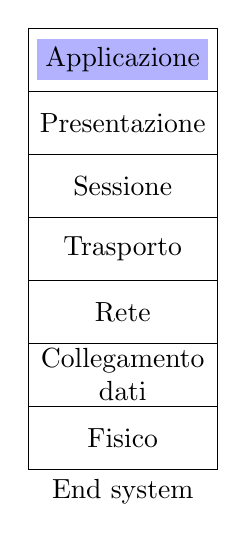
\begin{tikzpicture}[scale=0.8]
        \draw (0,6) rectangle ++(3,1) node[midway] {\colorbox{blue!30!white}{Applicazione}};
        \draw (0,5) rectangle ++(3,1) node[midway] {Presentazione};
        \draw (0,4) rectangle ++(3,1) node[midway] {Sessione};
        \draw (0,3) rectangle ++(3,1) node[midway] {Trasporto};
        \draw (0,2) rectangle ++(3,1) node[midway] {Rete};
        \draw (0,1) rectangle ++(3,1) node[midway,align=center] {Collegamento\\dati};
        \draw (0,0) rectangle ++(3,1) node[midway] {Fisico};
        \node[below] at (1.5,0) {End system};
      \end{tikzpicture}
    \end{figure}
Quando un messaggio (di qualsiasi tipo, che sia un email, frame di un video, richiesta/risposta HTTP) viene generato da un applicazione, si deve decidere quale protocollo utilizzare a livello di trasporto. \begin{itemize} \item 
\textbf{TCP} che sta per \textit{Transmission Control Protocol} (Connection Oriented e affidabile) oppure \item \textbf{UDP} che sta per\textit{ User Datagram Protocol } (Connectionless e Non affidabile)
\end{itemize}
Un servizio di trasporto più \textbf{affidabile} garantisce che la consegna arrivi a destinaizone.

\subsection{Esempi di applicazioni e relativi protocolli di trasporto}

Un esempio di protocollo di trasporto dati possono essere:

\begin{itemize}
    \item Web $\Longrightarrow$ \textbf{HTTP} $\Longrightarrow$ quando io invio un messaggio devo assicurarmi che non contenga errori, quindi il protocollo HTTP si appoggia al \textbf{TCP}.
    \item Posta elettronica $\Longrightarrow$ \textbf{SMTP} $\Longrightarrow$ anche'esso deve essere affidabile poiché non posso permettermi che l'email inviate possiedano errori.
    \item Streaming Audio/Video $\Longrightarrow$ Proprietari $\Longrightarrow$ Tollerante alle perdite $\Longrightarrow$ \textbf{UDP}
    \item \textbf{DNS} (Domain Name System) è il sistema che trasforma i nomi del dominio in indirizzi IP e l'esecuzione di questo sistema avviene attraverso il protocollo \textbf{UDP}.
\end{itemize}
Quando un applicazione deve mandare un messaggio ad un altra applicazione, \textit{"apre"} un \textbf{SOCKET} verso la destinazione.

\subsection{Socket}

\begin{definition}
\textit{Un socket è un'astrazione software che identifica un flusso informativo.}

Per \textit{aprire} un socket serve specificare le seguenti cose:
\begin{enumerate}
    \item Il \textit{protocollo di trasporto} utilizzato (TCP o UDP)
    \item Indirizzo IP di destinazione
    \item Indirizzo IP sorgente
    \item Porta di destinazione (processo)
    \item Porta sorgente 
\end{enumerate}
\end{definition}
Tra i due processi comunicanti possiamo identificare due ruoli distinti: 
\begin{enumerate}
    \item Il processo \textbf{CLIENT} \begin{itemize}
        \item È responsabile dell'apertura dell'inizio della comunicazione
        \item Ha un indirizzo \textit{dinamico}
    \end{itemize}
    \item Il processo \textbf{SERVER} \begin{itemize}
        \item Sta su un host sempre raggiungibile e sempre in ascolto
        \item Tipicamente ha un indirizzo IP \textit{fisso}
    \end{itemize}
\end{enumerate}

\subsection{Il protocollo HTTP}

Il protocollo HTTP (HyperText Transfer Protocol) è un protocollo di livello applicativo usato per la trasmissione di messaggi ipertestuali. Questo protocollo è di tipo \textbf{testuale} (i messaggi sono scritti in ASCII). Questo protocollo determiina il formato dei messaggi ed è basato sul modello \textbf{richiesta/risposta}.

\begin{enumerate}
    \item Il client apre un canale di comunicazione (Socket [5.2]), avvia un messaggio di richiesta e il server invia un messaggio di risposta.
    \item Il server mantiene nella pagina web $\rightarrow$ file di testo + altri contenuti. Il file di testo principale (\texttt{index.html}) contiene la struttura della pagina. Un file \texttt{html} definisce sia la struttura sia il contenuto di una pagina web.
\end{enumerate}
Il messaggio di richiesta è formato da 2 parti.
\begin{enumerate}
    \item Riga di richiesta
    \item Un o più righe di intestazione
\end{enumerate}

\begin{examplebox}{Esempio}
\texttt{GET /index.html/HTTP/1.1}\\
        \texttt{Host: www.univr.it\\
        User\_Agent: Mozilla/4.0\\
        Accept\_Language: en\\}
        \\
Corrisponde nel browser ad aver inserito:
\[
\texttt{wwww.univr.it/index.html}
\]
\end{examplebox}

\subsection{Metodi HTTP}

    \textit{\textbf{GET è una parola chiave che è definito come "metodo"}} dove andiamo a richiedere una pagina ad un server. \\
Tra gli altri metodi che esistono, vi è anche il \textit{\textbf{POST}}, che invia le informazioni al server. Un ulteriore metodo è \textit{\textbf{DELETE}} che serve per cancellare informazione/risorse sul server.

\subsection{Messaggio di risposta HTTP}

Come è strutturato un messaggio di risposta HTTP? 
\begin{enumerate}
    \item Riga di stato
    \item Una o più righe di intestazione
    \item Dati
\end{enumerate}

\begin{examplebox}{Esempio}
    \begin{center}
        \begin{itemize}
            \item \texttt{HTTP/1.1    codice\_di\_risposta   descrizione\_della\_risposta}
            \item  \texttt{Etichetta: valore}\\
            \item 
        \end{itemize}
Esempi di risposta e descrizione:
    \end{center}
\begin{align*}
    \colorbox{green!30!white}{200} & \; \; \text{OK}\\
    \colorbox{red!30!white}{404} & \; \;\text{NOT FOUND}\\
    \colorbox{yellow!40!white}{400} & \; \;\text{BAD REQUEST}
\end{align*}

\end{examplebox}

Per aprire una connessione su macchine \textit{Linux-based} si usa il comando \texttt{nc}.

\begin{lstlisting}
nc -vc indirizzo_url port
\end{lstlisting}


\subsection{Altri elementi del protocollo HTTP $\rightarrow$ COOKIE}

Meccanismo utilizzato dai server web per saper se ha interagito in passato con un determinato client. Non basta solo l'indirizzo IP per capire se un client ha interagito con un server. 
\\\\
I cookie sono delle coppie chiave-valore che vengono inviati dal server web al client (browser) attraverso l'intestazione HTTP della risposta. Quando il client riceve i cookie, li salva localmente e li invia automaticamente al server nelle successive richieste HTTP, a meno che non siano scaduti o non rientrino nei parametri di sicurezza stabiliti.
\\\\
I cookie servono principalmente a gestire sessioni e a memorizzare informazioni sullo stato dell'utente in un'applicazione web. Alcuni usi tipici includono:
\begin{itemize}
    \item \textbf{Autenticazione}: quando un utente effettua l'accesso a un sito, il server invia un cookie che identifica l'utente in modo da non dover eseguire il login a ogni nuova richiesta.
    \item \textbf{Personalizzazione}: salvare preferenze dell'utente, come la lingua preferita o il tema del sito.
    \item \textbf{Tracciamento}: possono essere usati per tenere traccia delle attività di navigazione dell'utente per fini analitici o pubblicitari.
\end{itemize}

\subsection{Caching}
Il \textit{caching} è un meccanismo per diminuire il ritardo per accedere ad una risorsa. Cache di rete è il ritardo nella consegna dei messaggi. Come sotto prodootto abbiamo che diminuisce il carico della rete.
\\\\
Una buona cache lavora con $70 - 80\%$ di cache hit.
\\\\
\textit{\textbf{Cne cosa succede se il contenuto nel server di origine cambia?}}
\\
Il protocollo HTTP prevede il meotdo GET-condizionale in cui una riga di intestazione della richiesta è \texttt{if\_modified\_since:<data>}.\\\\
Nella risposta del server (la prima con il contenuto o le successive con \texttt{not modified}) viene indicato anche il periodo di validità.

\subsection{DNS - Domain Name System}

Lo scopo principlae del DNS è la traduzione dei nomi logici come ad esempio \texttt{www.univr.it} nel corrispettivo indirizzo IP (ad esempio 157.25...).
\\\\
\textit{Come conosco l'indirizzo IP del server DNS?
}
\begin{itemize}
    \item[$\rightarrow$] Può essere inserito manualmente dall'utente nelle impostazioni
    \item[$\rightarrow$] Viene fornito dalla rete stessa quando viene assegnato l'indirizzo IP (DHCP)
\end{itemize}
\textit{Come fa  il DNS a conoscere per ciascun dominio, quindi per ciascuno nome logico presente su internet, conoscere l'assocazione tra il dominio e l'indirizzo IP (potenzialmente miliardi)?}\\\\
Non esiste un singolo server DNS ma c'è un sistema distribuito e gerarchico di server che si parlano tra di loro.

\begin{itemize}
    \item \textbf{Server DNS radice} (7-10): gestiscono le informazioni relativi ai domini di primo livello (.it, .fr, .com, ...)
    \item \textbf{Server DNS locali} gestiscono le informazioni relative ai domini di organizzazione specifica (univr.it, repubblica.it, ...)
\end{itemize}
In un indirizzo \textbf{URL:} 
\begin{center}
  \texttt{\colorbox{red!30!white}{www}.\colorbox{blue!30!white}{univr}.\colorbox{yellow!40!white}{it}}\\
  www = Server\\
  univr = Locali\\
  it = TLD
\end{center}
Il client interagisce solamente con il server DNS locale e con una serie di passaggi gli viene recuperato l'indirizzo IP da lui richiesto tramite l'indirizzo logico.\\
Il server DNS locale memorizza le risposte e quindi gli indirizzi IP dei server DNS TLD e server DNS locali con cui ha interagito recentemente.
\\\\
\textit{Qual è il rapporto tra DNS e Network Cache?}\\

\subsection{Protocolli di posta elettronica}

\begin{itemize}
    \item Invio \begin{itemize}
        \item[$\rightarrow$] SMTP (Simple Mail Transfer Protocol)
    \end{itemize}
    \item Ricezione \begin{itemize}
        \item[$\rightarrow$] POP (Non più utilizzato) (Post Office Protocol)
        \item[$\rightarrow$] IMAP (Internet Mesage Access Protocol)
        \item[$\rightarrow$] HTTP (Webmail)
     \end{itemize}
\end{itemize}
Tutti i protocolli si appoggiano su TCP. Dal punto di vista dell'architettura ogni dominio di posta elettronica (la porzione che segue la \@ dell'indirizzo di posta elettronica) deve avere associato uno specifico server SMTP che gestisce le caselle degli utenti appartenenti a quel dominio.\\
Quando il server univr.it riceve un messaggio, controlla il dominio, se il dominio è \texttt{univr.it}, allora mette il messaggio sulla corrispondente casella di posta. Se il dominio è diverso, il server SMTP controlla il server SMTP di destinazione per la consegna del messaggio attraverso il protocollo SMTP.

\pagebreak

\section{Livello di Trasporto}

\subsection{Header del protocollo TCP}

L'header del protocollo TCP (Transmission Control Protocol) è una parte fondamentale del protocollo, che viene utilizzata per gestire la trasmissione affidabile dei dati tra due dispositivi su una rete. Ogni segmento TCP, ovvero ogni unità di dati inviata, contiene un header che include informazioni necessarie per la corretta gestione e interpretazione della connessione e dei dati.
\\
L'header TCP standard è composto da 20 byte (minimo) e può essere esteso con campi opzionali. Vediamo i campi principali:
\begin{itemize}
	\item[$\rightarrow$] \textbf{Porta Sorgente/Destinazione}: Indentificatori dei processi sorgente e destinazione coinvolti nella comunicazione. Esistono due tipi di porte:
	\begin{itemize}
		\item Statiche, ovvero sono i numeri di porte che vanno da 0 - 1023, identificativi associati a protocolli definiti dallo standard (HTTP, SMTP, \dots) utilizzati \textbf{lato server}.
		\item Dinamiche, $\ge 1024$ e sono identificativi assegnati dal sistema operativo \textbf{lato client} quando viene aperto un socket.
\end{itemize}

\item[$\rightarrow$]\textbf{Numero di sequenza}, numero sequenziale che identifica univocamente ogni byte di dati nel flusso TCP.
È cruciale per il riordinamento dei pacchetti, specialmente se alcuni di essi vengono ricevuti fuori ordine.		
\begin{itemize}
		\item A livello applicativo vengono generati messaggi di dimensione arbitraria
		\item A livelllo ``Collegamenti Dati'' (L2) alla scheda di rete è associato un parametro chiamato:
			\begin{itemize}
				\item MTU Maximum Transmission Unit
				\item MSS Maximum Sequent Size
			\end{itemize}
	\end{itemize}
\item[$\rightarrow$] \textbf{Numero di riscontro o di acknowledgment\footnote{ACK: È un segmento TCP senza dati (Solo header)}}: Questo campo è utilizzato per confermare la ricezione dei pacchetti. Contiene il numero di sequenza del byte successivo che il ricevente si aspetta di ricevere.
L'uso del numero di riscontro rende possibile il controllo di flusso e la conferma di ricezione dei dati.
\item[$\rightarrow$] \textbf{Checksum}, 
serve per controllare la presenza di errori nel segmento. La checksum è 
il risultato di una funzione che prende in input il 
segmento e restituisce un valore a dimensione fissa 
univoco per quel segmento. Se il segmento viene modificato 
durante la trasmissione, la checksum cambia e il destinatario fa 
un controllo mettendo in input ciò che ha ricevuto e se il confronto:
\begin{itemize}
  \item Va a buon fine: con \textbf{alta probabilità} non ci sono stati errori
  \item Non a buon fine: ci sono \textbf{sicuramente} degli errori
\end{itemize}

\end{itemize}

\subsubsection{Gestione delle connessioni}
TCP è un protocollo connection oriented, cioè prima di scambiare dati, client 
e server devono stabilire che vogliono comunicare e questo avviene tramite 
l’invio di messaggi di servizio (senza dati), questa fase è chiamata 
instaurazione della connessione.
\\\\
\textbf{N.B.:} Instaurare una connessione non ha niente a che fare con la creazione di un circuito o riservare delle risorse di rete
\\\\
Quindi avviene uno scambio di segmenti TCM (header senza payload) chiamata \textit{Three-way handshake}:
\begin{itemize}

  \item \textbf{Syn}: Il client invia un segmento con il flag SYN a 1. Questo segmento contiene l’initial sequence number del client (ISN), cioè un numero scelto casualmente da cui il client inizia a numerare i byte inviati. Questo numero serve anche come ulteriore sicurezza per la cifratura.
  \item \textbf{Syn-Ack}: Il server risponde con un segmento con i flag SYN e ACK a 1. Questo segmento contiene l’initial sequence number del server e l’acknow- ledgment number uguale all’ISN del client + 1.
  \item \textbf{Ack}: Il client risponde con un segmento con il flag ACK a 1 e l’acknow- ledgment number uguale all’ISN del server + 1.
  \item \textbf{Altri parametri}: MSS (Maximum Segment Size): Indica la dimensione massima di un segmento che il client e il server possono ricevere. Client e server utilizzeranno il valore minimo tra le 2 MSS comunicate. La MSS è contenuta nelle opzioni dell’header TCP, che sono utilizzate solo se necessario.
\end{itemize}
Dopo aver instaurato la connessione gli host si possono scambiare i messaggi: Quando lo scambio dei messaggi è terminato, la connessione viene chiusa attra- verso uno scambio di header. Siccome il canale è biirezionale, la chiusura deve avvenire indipendentemente nelle due direzioni. I 2 messaggi sono:
\begin{itemize}
  \item \textbf{FIN}: sarà un messaggio con il flag \texttt{FIN} a 1.
  \item \textbf{ACK}: sarà un messaggio con il flag \texttt{ACK} a 1.
\end{itemize}
TCP è un protocollo affidabile, cioè quando un host invia un segmento si aspetta di ricevere il riscontro entro un tempo massimo (RTO, Retransmission Ti- meOut). L’RTO dovrà tenere in conto l’RTT (Round Trip Time), cioè il tempo che impiega un segmento a viaggiare da un host all’altro e tornare indietro.

\subsubsection{RTO e RTT}

L'RTO dipende dal valore del RTT (Round Trip Time $\rightarrow$ tempo che impiega un segmento a 
viaggiare da un host all'altro e tornare indietro.). All'apertura della connessione, misura il RTT
durante il Three-way handshake. Per l'invio del primo messaggio (Syn) l'RTO è impostato a 500 ms.
\\\\
\textit{Come vengono aggiornati i valori di RTT e RTO?}
 Ogni Host, per ongi segmento inviato, misuro l'RTT instantaneo e usa tale valore per aggiornare una variabile
 chiamata: \textit{SRTT $\rightarrow$ Smoothed Round Trip Time}.
\[SRTT_{attuale} = \alpha SRTT_{precedente} + (1 - \alpha)RTT_{instantaneo}\]
\[0 < \alpha < 1\]
L'SRTT è uno \textbf{stima} del valore medio del RTT. Questa tecnica si chiama \textit{Exponential Weighted Moving Average} (EWMA).
\\ Dato l'SRTT: \[RTO = \beta SRTT_{attuale}\]dove tipicamente $\beta = 2$. Quindi in poche parole, il segmento viene
ritrasmesso dopo un tempo pari al doppio del tempo medio di ritorno. In caso di perdite, l'RTO per il segmento
ritrasmesso  viene temporaneamente raddoppiato. Se invio un segmento ad ogni RTT, la velocità di trasmissione
è  $\frac{1 seg}{k\pi} \rightarrow \frac{1500 byte}{100ms} = 1200$ byte/sec.

\subsection{Controllo di flusso e il controllo di congestione}

Per aumentare la velocità di trasmissione invece di trasmettere un singolo segmento ne trasmetto di più contemporaneamente. Per esempio, se ne inviassi
due alla volta, raddoppierai la velocità di trasmissione. Tuttavia questo genera diversi problemi. Come gestisco i riscontri
e cosa succede se uno dei segmenti viene perso? Ci sono due tecniche che ci aiutano in questo caso:

\begin{enumerate}
  \item Il controllo di flusso $\rightarrow$ Azione preventiva per limitare la congestione. 
  Inviare più segmenti contemporaneamente con un meccanismo o finestra scorrevole
  \item Il controllo di congestione $\rightarrow$ Reazione in caso di congestione
\end{enumerate}
\begin{center}
  Congestione $\Longleftrightarrow$ Perdita di un segmento (Riscontro non ricevuto)
\end{center}
Grazie all'ACK che mi dice quale è il prossimo segmento che si aspetta, posso essere sicuro di non perdere i pacchetti ed 
essere ancora più affidabile.
Quant'è la dimensione della finestra di trasmissione? Utilizzzare i riscontri (o la loro assenza) per variare in modo dinamico la window size.
\begin{itemize}
  \item Se ricevo regolarmente i riscontri, aumento la finestra di trasmissione
  \begin{itemize}
    \item Slow Start
    \item Congestion Avoidance
  \end{itemize}
  \item In caso di perdite (RTO scende), diminuisco la finestra di trasmissione 
  \begin{itemize}
    \item Vanilla 
    \item Fast Retransmit/Fast Recovery
  \end{itemize}
\end{itemize}

\subsubsection{Slow Start}

Per ogni riscontro ricevuto si fa aumenta la finestra di un segmento. (Oltre a farla scorrere verso destra di un segmento).

\begin{tikzpicture}
  \begin{axis}[
      axis lines=middle,
      xlabel={$t$},
      ylabel={$w$},
      xtick={1,2,3},
      ytick={2,4,8,16},
      ymin=0, ymax=18,
      xmin=0, xmax=3.5,
      axis line style={->},
      every axis x label/.style={
          at={(ticklabel* cs:1.05)},
          anchor=west,
      },
      every axis y label/.style={
          at={(ticklabel* cs:1.05)},
          anchor=south,
      }
  ]
  
  % Draw the plot and points
  \addplot[thick, mark=*] coordinates {(0,2) (1,4) (2,8) (3,16)};
  
  % Add labels for each point
  \node[anchor=south] at (axis cs:0,2) {2};
  \node[anchor=south] at (axis cs:1,4) {4};
  \node[anchor=south] at (axis cs:2,8) {8};
  \node[anchor=south] at (axis cs:3,16) {16};
  
  % Dashed line upwards for future points
  \draw[dashed] (axis cs:3,16) -- (axis cs:3.5,18);
  
  \end{axis}
\end{tikzpicture}


\subsubsection{Congestion Avoidance}

Per ogni riscontro ricevuto, aumento la finestra di $1/w$ dove $w$ è la dimensione precedente della finestra.



\begin{tikzpicture}
  \begin{axis}[
      axis lines=middle,
      xlabel={$t$},
      ylabel={$w$},
      xtick={1,2,3},
      ytick={2,4,8,16},
      ymin=0, ymax=18,
      xmin=0, xmax=3.5,
      axis line style={->},
      every axis x label/.style={
          at={(ticklabel* cs:1.05)},
          anchor=west,
      },
      every axis y label/.style={
          at={(ticklabel* cs:1.05)},
          anchor=south,
      }
  ]
  
  % Draw the plot and points
  \addplot[thick, mark=*] coordinates {(0,2) (1,3) (2,4) (3,5)};
  
  % Add labels for each point
  \node[anchor=south] at (axis cs:0,2) {2};
  \node[anchor=south] at (axis cs:1,3) {3};
  \node[anchor=south] at (axis cs:2,4) {4};
  \node[anchor=south] at (axis cs:3,5) {5};
  
  % Dashed line upwards for future points
  \draw[dashed] (axis cs:3,5) -- (axis cs:4,6);
  
  \end{axis}
\end{tikzpicture}



\subsubsection{Vanilla}

Se non arriva il riscontro, si attende lo scadere del RTO, si pone la finestra = 1 e si ritrasmettono i segmenti persi.

\subsubsection{Fast Retransmit/Fast Recovery}

In caso di ricezione di ACK duplicati, dopo averne ricevuti 3, si pone la finestra a $w' = \frac{w}{2} \leftarrow$ (finestra al momento della perdita) e
si ritrasmette il segmento indicato negli ACK duplicati. (E se ci sono le "opzioni" presenti che indicano gli altri segmenti
segmenti mancanti, si ritrasmettono anche quelli).

\subsubsection{Algoritmo di controllo della congestione del TCP}

Variabili: 
\begin{itemize}
  \item \textbf{CWND} $\rightarrow$ Congestion Window $\rightarrow$ dimensione di trasmissione attuale 
  \item \textbf{RTO} $\rightarrow$ Calcolo dinamicamente in base all'RTT instantaneo e SRTT.
  \item \textbf{RCVWND} $\rightarrow$ Receive Window $\rightarrow$ Finestra massima di ricezione 
  \item \textbf{SSTHRESH} $\rightarrow$ Slow Start Threshold $\rightarrow$ Soglia usata per distinguere Slow Start e Congestion Avoidance 
\end{itemize}

\begin{lstlisting}[language=Scala]
// Inizializzazione
CWND = 1
RCVWND = Viene caricato dalla destinazione in ogni riscontro
STTHRESH = RCVWND (in alcune implementazioni (RCVWND/2))
RTO = in base a valore del RTT misurato nel 3-way-handshake
// Algoritmo
1 . Invia un numero di seguenti pari alla CWND
2. Quando arrivano i riscontri
  if CWND < SSTHRESH // uso slow_start
    CWND = min(CWND + #ack, RCVWND, STTHRESH)
  else               // uso Congesture Avoidance
    CWND = CWND + (#ack/CWND)
Torno al punto 1. 
3. Se non arrivano i riscontri -> Scade il RTO
pongo la STTHRESH = CWND al momento della perdita/2 
pongo la CWND = 1 // Variante Vanilla TCP
per i segmenti ritrasmessi pongo RTO = 2RTO
Torno al punto 1. 
    
\end{lstlisting}
Esempio dell'evoluzione della trasmissione TCP (semplificato poiché siamo nel caso RTT sia mediamente stabile)

\subsection{Protocollo UDP (User Datagram Protocol)}

Il protocollo UDP:
\begin{itemize}
  \item Connectionless: Non c'è uno scambio preliminare prima di inviare i dati, ed è anche \textbf{non affidabile}
  cioè se i segmenti vengono persi non vengono ritrasmessi. 
  \item Non affidabile: in caso di perdita, i segmenti \textit{non} vengono ritrasmessi
\end{itemize}

\subsubsection{Header del protocollo UDP}

Le particolarità del suo header è che contiene soltanto:
\begin{itemize}
  \item Porta Sorgente
  \item Porta destinazione
  \item Lunghezza (del messaggio)
  \item Checksum, serve per controllare gli errori nel segmento
\end{itemize}
Possiamo notare come non è presente il sequence number, infatti non consegna i segmenti in ordine che 
vengono inviati dal livello applicativo. Proprio per questo, il protocollo è molto leggero durante
la trasmissione di dati in tempo reale, infatti non carica molto il processore essendo
che non deve gestire efficaciamente i dati.

\pagebreak

\section{Livello di Rete}

\subsection{Il protocollo IP (Internet Protocol)}

\subsubsection{Header dell'IP}
L'header del protocollo IP contiene le seguenti specifiche:

\begin{itemize}
  \item Versione del protocollo, indica la versione del protocollo IP utilizzato. Attualmente la versione che usiamo è IPv4 ma nel futuro si utilizzerà IPv6
  \item Lunghezza dell'header $\rightarrow$ 20 byte se non ci sono opzioni può essere più lungo
  \item Service Type $\rightarrow$ Codice che identifica una classe del servizio
  \item Lunghezza totale del pacchetto $\rightarrow$ Header + Payload
  \item Identification, flag e Fragment Offset $\rightarrow$ Usati per la frammentazione dei pacchetti
  \item Time to Live $\rightarrow$ Numero di hop massimi che il pacchetto può fare (Max 64 Router) ogni volta che attraversa un Router il valore viene decrementato di uno
  se il valore diventa 0, manda un messaggio di errore alla sorgente e scarta il pacchetto. In caso di problemi
  di routing, la rete deve ricalcolare il percorso e nel frattempo si possono creare dei routing-loop. (momentanei)
  \item Type $\rightarrow$ Codice che identifica il protocollo di trasporto (TCP, UDP, ICMP, \dots) 
  \item Header Checksum $\rightarrow$ Controllo degli errori dell'header
\end{itemize}

\subsubsection{Frammentazione IP}

Data una tecnologia di trasmissione (Scheda di rete, a livello datalink) c'è una dimensione massima
di trasmissione chiamata MTU. \\
Che cosa succede se un pacchetto durante il percorso incontra una MTU minore di quella del pacchetto?
\textit{Il pacchetto viene frammentato in pacchetti più piccoli}.

\begin{itemize}
  \item[$\rightarrow$] Il \textit{router} con link di uscita con MTU $<$ dimensione del pacchetto, frammenta il pacchetto in più pacchetti con MTU
  compatibile con il link di uscita.
\end{itemize}
I campi dell'header coninvolti nella frammentazione sono:
\begin{itemize}
  \item \textbf{Identification} $\rightarrow$ Numero progressivo dato dalla sorgente (livello di rete) ad ogni pacchetto (nessuna relazione con il \# sequenza del TCP)
  \item \textbf{Flag} $\rightarrow$ 3 bit: \begin{itemize}
    \item $\rightarrow$ Bit "M", se il pacchetto non è stato frammentato 0 oppure se è l'ultimo frammento.
    altrimenti 1 se il pacchetto è un frammento tranne l'ultimo
  \end{itemize}
  \item \textbf{Fragment Offset} $\rightarrow$ Indica la posizione del frammento all'interno del pacchetto originale (diviso per 8.)

\end{itemize}
\begin{examplebox}{Esempio}
  MTU $= 1500$ byte, pacchetto $= 4000$ byte $+ 20$ byte header IP.

  Nel percorso, il pacchetto passa attraverso un router con link di uscita:
  \begin{itemize}
    \item 1400 byte per il payload
    \item 20 byte per l'header IP
  \end{itemize}

  Quindi posso dividere il pacchetto fino ad un max di 3 frammenti, 2 da 1400 byte e 1 da 1200 byte.\\\\
  \textbf{Identification}: Avranno lo stesso ID del pacchetto originario.\\
  \textbf{Flag}: Per quanto riguarda la flag del primo frammento, il bit M sarà 1, per gli altri 0.\\
  \textbf{Fragment Offset}: $\text{Frammento 1} = 0, \; \text{Frammento 2: } \frac{1400}{8} = 175, \; \text{Frammento 3: } \frac{2800}{8} = 350$
  \end{examplebox}

  Chi fa il riassemblaggio?
  \begin{itemize}
    \item Il riassemblaggio viene fatto dal destinatario (host finale) e non dai router. 
    \item Quando la destinazione riceve un frammento fa partire un timer (250-500 ms) per attendere gli altri frammenti. Se li riceve entro 
    la scadenza del timer procede con il riassemblaggio, altrimenti scarta i frammenti ricevuti.
  \end{itemize}


\subsection{Routing / Instradamento}

Scopo del livello di rete: Data una destinazione $\overbrace{\text{fare il possibile}}^{\text{best effort}}$ per consegnare il pacchetto al destinatario.
Quindi per fare in modo che il pacchetto arrivi a destinazione bisogna effettuare il routing (instradamento) del pacchetto.

\subsubsection{Consegna diretta/indiretta}

Un host conosce, oltre al proprio indirizzo IP, la maschera della rete a cui appartiene e l'indirizzo IP (dell'interfaccia) del router di bordo. 
\\
Data una destinazione ($IP_d$) l'host confronta $\overbrace{\text{IP e Maschera}}^{\text{prefisso immutato e suffisso a 0}}$
e $IP_d$ e maschera. Se i due valori \textbf{sono uguali} la destinazione appartiene alla stessa rete e quindi avviene la \textbf{consegna diretta}.
Altrimenti vuol dire che la destinazione appartiene ad un'altra rete e quindi faccio la \textbf{consegna indiretta} ovvero \textit{demando la consegna al router}.

\begin{definition}
  Il \textit{routing} è un processo di scoperta del cammino "migliore" da una sorgente a tutte le possibili destinazioni. 
\end{definition}
\noindent
"Migliore" perché tutto ciò dipende dai criteri adottati da chi gestisce la rete (ISP).
\begin{examplebox}{Esempio}
  Tipi di criteri: 
  \begin{itemize}
    \item Distanza (cammino più corto), in termini di numero di hop (\# router attraversati) o in termini di chilometri.
    \item Velocità di trasmissione
    \item Livello di congestione (ma che non viene utilizzato)
\end{itemize}
\end{examplebox} 
\noindent
Data la rappresentazione dei grafi della rete (dove gli archi hanno associato un costo), \textit{il routing} non è altro che il \textbf{calcolo del cammino con il costo minimo}.
Chi ha già conoscenza nel campod degli algoritmi questo tipo di approccio è conososciuto come \textit{Shortest Path Problem} e vengono applicati 
algoritmi di Pathfinding.

\vspace{1em}
\noindent
Dato una topologia (router e collegamenti) derivo il grafo e assegno i pesi secondo un criterio:
\begin{itemize}
  \item \# di hop $\rightarrow$ Tutti gli archi hanno peso 1
  \item velocità di trasmissione (capacità nominale del link) i pesi sono proporzionale all'inverso della banda
\end{itemize}
Algoritmi per il calcolo del cammino minimo:
\begin{itemize}
  \item Stato dei collegamenti: Link-State
  \item Vettori di distanza: Distance-Vector
\end{itemize}


\subsection{Algoritmi di link-state}
\begin{itemize}
  \item Ogni nodo ha una tabella di routing
  \item Ogni nodo conosce la topologia della rete
  \item Ogni nodo calcola il cammino più breve verso tutti gli altri nodi
\end{itemize}
Ad ogni algoritmo corrisponde un protocollo di routing. Protocllo basato su link-state: OSPF (Open Shortest Path First). 
\subsubsection{Algoritmo di Dijkstra}

\begin{definition}
  L'algoritmo di Dijkstra è un algoritmo che permette di trovare il cammino più breve tra due nodi di un grafo pesato, con pesi non negativi.
\end{definition}
\noindent
I nodi si riscambiano i messaggi (Questi messaggi trasportano informazioni sulla topologia della rete.)
\begin{enumerate}
  \item periodici, per controllare se sono ancora raggiungibili
  \item in caso di guasti/cambio di topologia
\end{enumerate}




\end{document}